%------------------------
% Resume Template
% Author : Anubhav Singh
% Github : https://github.com/xprilion
% License : MIT
%------------------------

\documentclass[a4paper]{article}

\usepackage{latexsym}
\usepackage[empty]{fullpage}
\usepackage{titlesec}
\usepackage{marvosym}
\usepackage[usenames,dvipsnames]{color}
\usepackage{verbatim}
\usepackage{enumitem}
\usepackage[pdftex]{hyperref}
\usepackage{fancyhdr}
\usepackage{fontawesome}
\usepackage{tabularx}
\usepackage{ulem}
\usepackage{graphicx}
\usepackage{ragged2e}
\usepackage{csquotes}

\pagestyle{fancy}
\fancyhf{} % clear all header and footer fields
\fancyfoot{}
\renewcommand{\headrulewidth}{0pt}
\renewcommand{\footrulewidth}{0pt}

\newcolumntype{C}{>{\centering\arraybackslash}X} % centered version of 'X' col. type

\raggedbottom
\raggedright
\setlength{\tabcolsep}{0in}

% Sections formatting
\titleformat{\section}{
  \scshape\raggedright\large
}{}{0em}{}[\color{black}\titlerule]

%-------------------------
% Custom commands
\newcommand{\resumeSubheading}[4]{
  \vspace{-1pt}\item
    \begin{tabular*}{0.97\textwidth}{l@{\extracolsep{\fill}}r}
      \textbf{#1}, #2 & \textit{#3} \\
    \end{tabular*}
    #4
}

\newcommand{\resumeSubheadingSimple}[2]{
  \vspace{-1pt}\item
	\begin{tabular*}{0.97\textwidth}{l@{\extracolsep{\fill}}r}
	  #1 & \textit{#2} \\
	\end{tabular*}
  \vspace{-1pt}
}

\newcommand{\resumeSubheadingVerySimple}[1]{
	\vspace{-1pt}\item #1
	\vspace{-1pt}
}

\newcommand{\resumeSubheadingItem}[1]{
  \vspace{0pt}\item #1
  \vspace{0pt}
}

\newcommand{\resumeSubHeadingListStart}{\begin{itemize}[leftmargin=*]}
\newcommand{\resumeSubHeadingListEnd}{\end{itemize}}

%-----------------------------
%%%%%%  CV STARTS HERE  %%%%%%

\begin{document}

\begin{center}
	\begin{tabular}{p{0.3\textwidth} p{0.4\textwidth} p{0.3\textwidth}}
		\raisebox{-0.7\height}{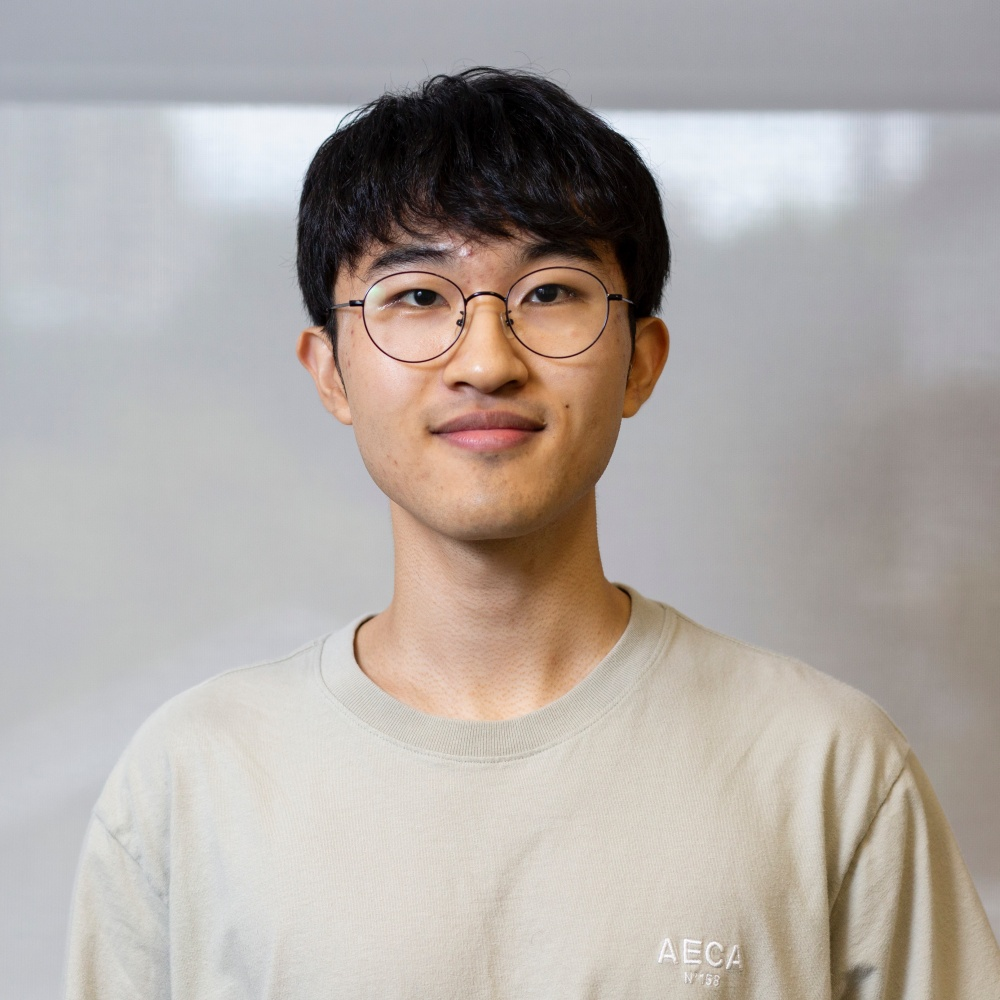
\includegraphics[width=0.3\textwidth]{../info/photo.jpg}} &
		\centerline{\textbf{{\LARGE Hyoungjoo Kim}}}
		\vspace{20pt}
		\centerline{\href{mailto:hyoungjoo@cmu.edu}{hyoungjoo@cmu.edu}}
		\vspace{10pt}
		\centerline{\url{https://hyoungjook.github.io}}
		\vspace{10pt}
		\centerline{
			\LARGE
			\href{https://scholar.google.com/citations?user=sYhlQ1YAAAAJ&hl=en}{\faicon{graduation-cap}} \quad
			\href{https://www.linkedin.com/in/hyoungjoo-kim-546986194}{\faicon{linkedin}} \quad
			\href{https://github.com/hyoungjook}{\faicon{github}}
		} & \\
	\end{tabular}
\end{center}

\input{info.tex}

\end{document}
